% This LaTeX was auto-generated from MATLAB code.
% To make changes, update the MATLAB code and export to LaTeX again.

\documentclass{article}

\usepackage[utf8]{inputenc}
\usepackage[T1]{fontenc}
\usepackage{lmodern}
\usepackage{graphicx}
\usepackage{color}
\usepackage{hyperref}
\usepackage{amsmath}
\usepackage{amsfonts}
\usepackage{epstopdf}
\usepackage[table]{xcolor}
\usepackage{matlab}

\sloppy
\epstopdfsetup{outdir=./}
\graphicspath{ {./lab1_images/} }

\begin{document}

\matlabtitle{1 - Getting Started}

\begin{par}
\begin{flushleft}
Load the data that we will use.
\end{flushleft}
\end{par}

\begin{matlabcode}
I = imread('lab1/images/napoleon.png');
Il = imread('lab1/images/napoleon_light.png');
Id = imread('lab1/images/napoleon_dark.png');
Z = imread('lab1/images/zebra.png');
\end{matlabcode}


\matlabheading{2 - Viewing Images and Saving Images}

\begin{par}
\begin{flushleft}
Below is one of the example images we will work on.
\end{flushleft}
\end{par}

\begin{matlabcode}
imtool(I);
\end{matlabcode}
\begin{center}
\includegraphics[width=\maxwidth{44.65629703963874em}]{figure_0.png}
\end{center}


\matlabheading{2 - Image Tool}

\begin{matlabcode}
imtool(I);
\end{matlabcode}
\begin{center}
\includegraphics[width=\maxwidth{44.65629703963874em}]{figure_1.png}
\end{center}


\matlabheading{Q1 - Pixel Value}

\begin{par}
\begin{flushleft}
Print out value. We see that it is of type UINT-8 and 
\end{flushleft}
\end{par}

\begin{matlabcode}
I(1, 1)         % It prints out 89
\end{matlabcode}
\begin{matlaboutput}
ans = 89
\end{matlaboutput}


\matlabheading{3 - Contrast, Brightness and Datatypes}

\begin{par}
\begin{flushleft}
Plot all three different example images. Regular, light and dark.
\end{flushleft}
\end{par}

\begin{matlabcode}
imtool(I);
imtool(Il);
\end{matlabcode}
\begin{center}
\includegraphics[width=\maxwidth{44.65629703963874em}]{figure_2.png}
\end{center}
\begin{matlabcode}
imtool(Id);
\end{matlabcode}
\begin{center}
\includegraphics[width=\maxwidth{44.65629703963874em}]{figure_3.png}
\end{center}
\begin{center}
\includegraphics[width=\maxwidth{44.65629703963874em}]{figure_4.png}
\end{center}


\matlabheading{Q2 - Histograms}

\begin{par}
\begin{flushleft}
From figure 1, which is the regular image, we see that the pixel values are spread across the domain $0,255$. The second figure is skewed towards the lighter pixel values and this image should be the high contrast one. The third histogram shows the third image and how it is skewed in the other direction and is thus the histogram of the low contrast image.
\end{flushleft}
\end{par}

\begin{matlabcode}
figure(1);
imhist(I);
\end{matlabcode}
\begin{center}
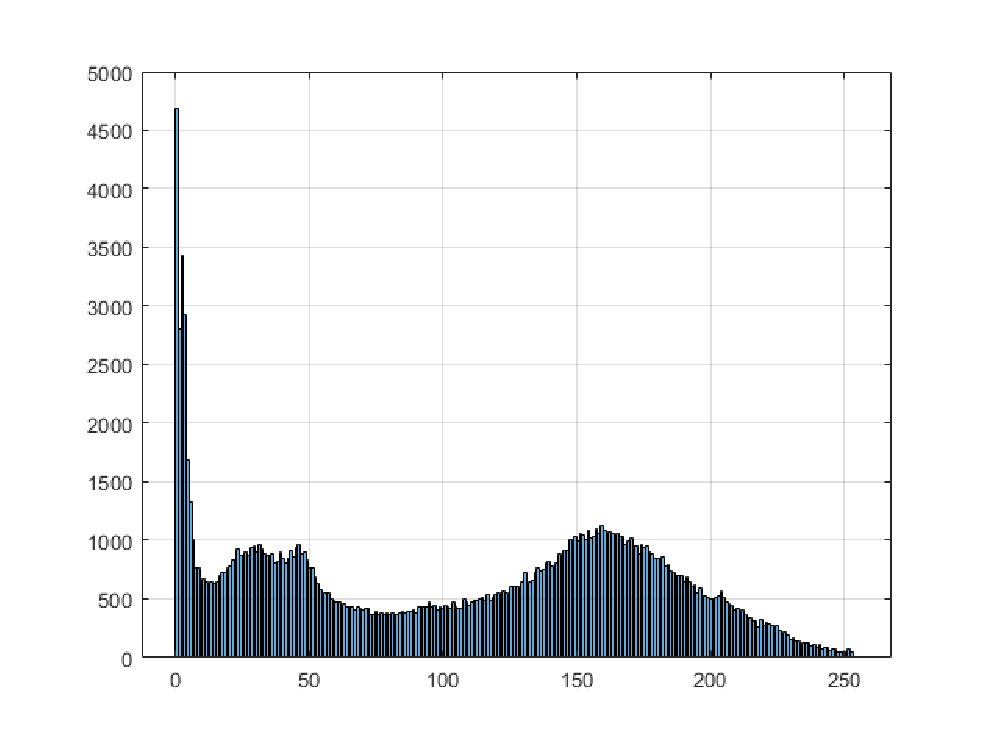
\includegraphics[width=\maxwidth{56.196688409433015em}]{figure_5.eps}
\end{center}
\begin{matlabcode}

figure(2);
imhist(Il);
\end{matlabcode}
\begin{center}
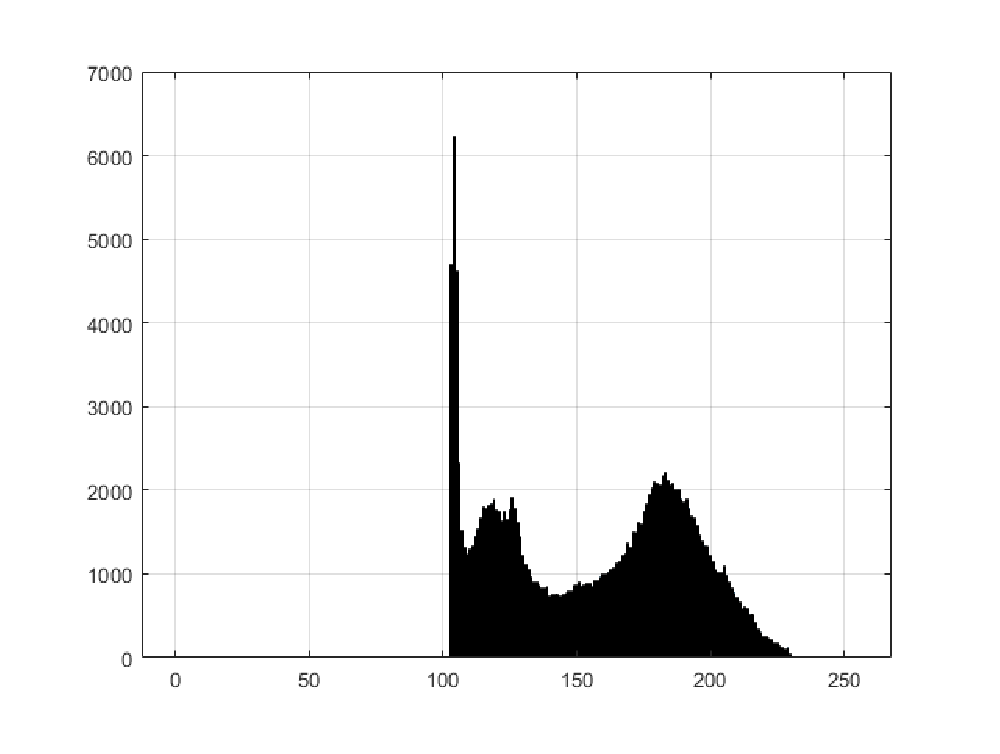
\includegraphics[width=\maxwidth{56.196688409433015em}]{figure_6.eps}
\end{center}
\begin{matlabcode}

figure(3);
imhist(Id);
\end{matlabcode}
\begin{center}
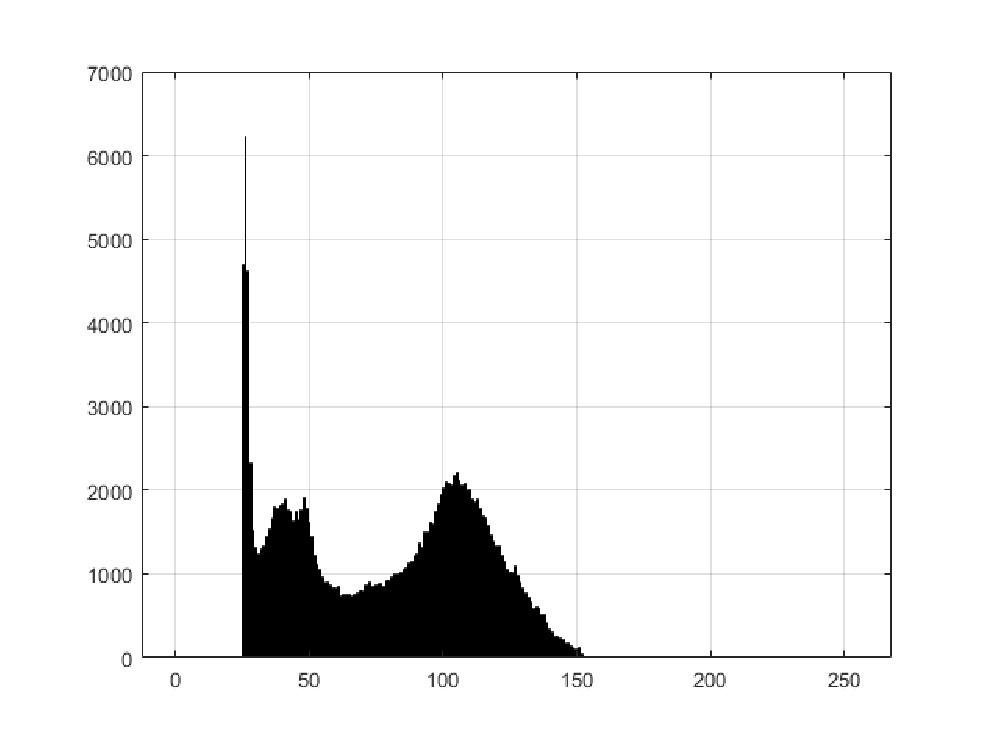
\includegraphics[width=\maxwidth{56.196688409433015em}]{figure_7.eps}
\end{center}


\matlabheading{See images}

\begin{matlabcode}
Is = single(I);
imtool(I);
imtool(Is);
\end{matlabcode}
\begin{center}
\includegraphics[width=\maxwidth{44.65629703963874em}]{figure_8.png}
\end{center}
\begin{matlabcode}
imtool(Is/255);
\end{matlabcode}
\begin{center}
\includegraphics[width=\maxwidth{44.65629703963874em}]{figure_9.png}
\end{center}
\begin{center}
\includegraphics[width=\maxwidth{44.65629703963874em}]{figure_10.png}
\end{center}


\matlabheading{Q3 - Explain differences}

\begin{matlabcode}
figure(1);
imtool((I/64)*64);

figure(2);
imtool((Is/64)*64);
\end{matlabcode}
\begin{center}
\includegraphics[width=\maxwidth{44.65629703963874em}]{figure_11.png}
\end{center}
\begin{center}
\includegraphics[width=\maxwidth{44.65629703963874em}]{figure_12.png}
\end{center}


\matlabheading{Q4 - Make images brighter}

\begin{matlabcode}
imtool(I + 50);
imtool(I);
\end{matlabcode}
\begin{center}
\includegraphics[width=\maxwidth{44.65629703963874em}]{figure_13.png}
\end{center}
\begin{center}
\includegraphics[width=\maxwidth{44.65629703963874em}]{figure_14.png}
\end{center}


\matlabheading{Q5 - Make images lower contrast}

\begin{matlabcode}
imtool(I);
imtool(I * 0.5);
\end{matlabcode}
\begin{center}
\includegraphics[width=\maxwidth{44.65629703963874em}]{figure_15.png}
\end{center}
\begin{center}
\includegraphics[width=\maxwidth{44.65629703963874em}]{figure_16.png}
\end{center}


\matlabheading{Q6 - Pixel Wise Transforms}

\begin{matlabcode}
figure(1);
imhist(I);

figure(2);
imshow(I);
\end{matlabcode}
\begin{center}
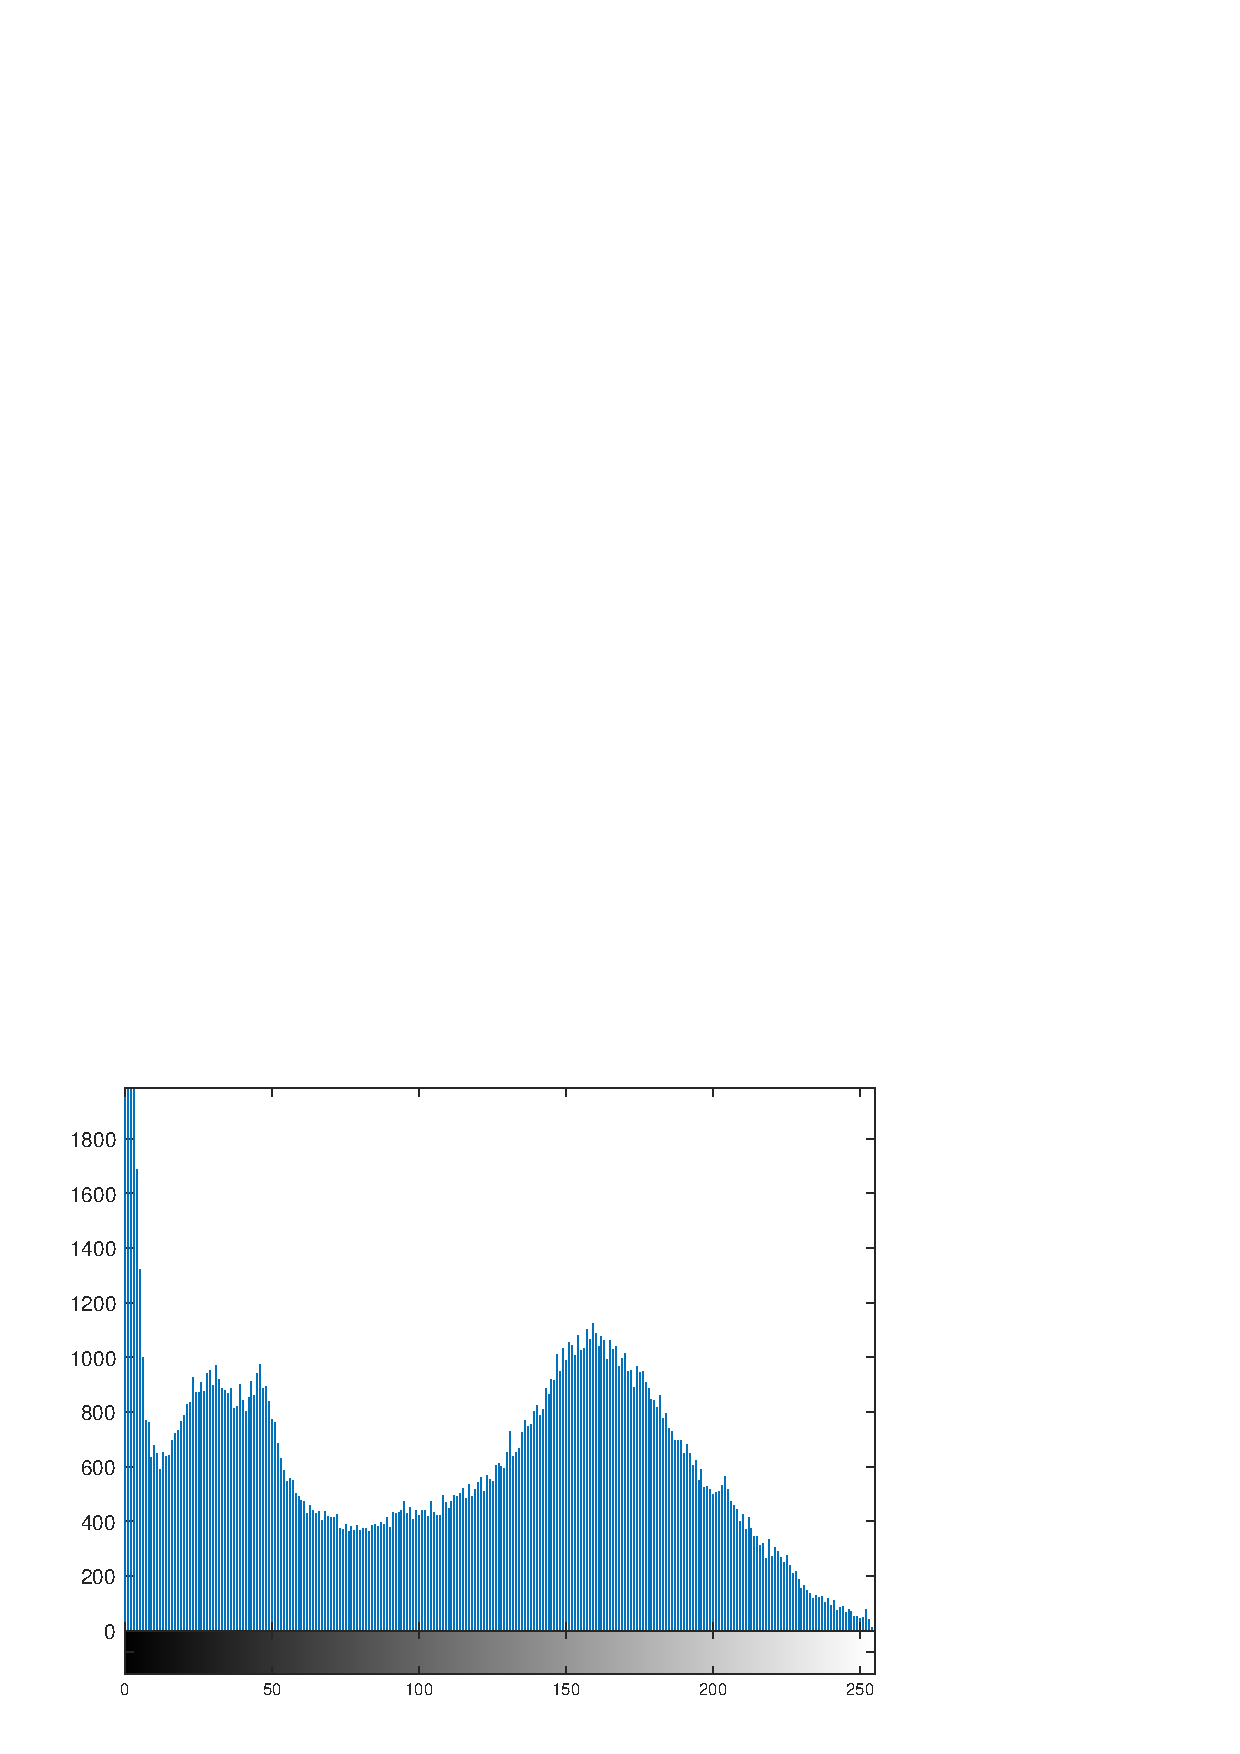
\includegraphics[width=\maxwidth{56.196688409433015em}]{figure_17.png}
\end{center}
\begin{matlabcode}

g = 0.5;
L = double(I).^g;
out = uint8(L .* (255/max(max(L))));

figure(3);
imhist(out);

figure(4);
imshow(out);
\end{matlabcode}
\begin{center}
\includegraphics[width=\maxwidth{62.117410938283996em}]{figure_18.png}
\end{center}
\begin{center}
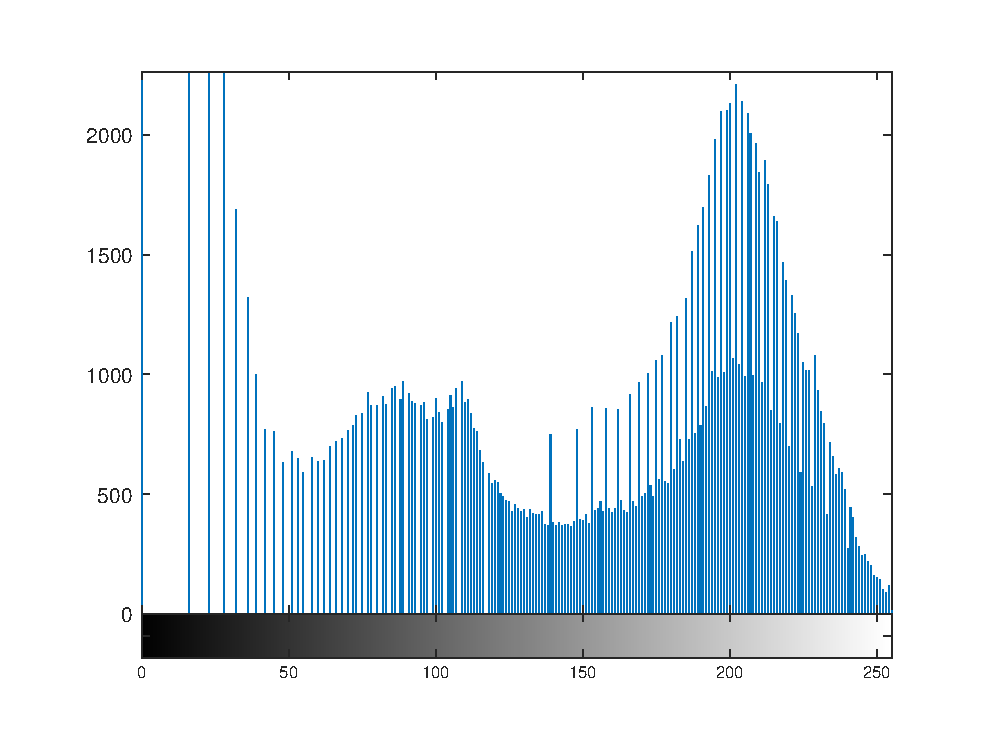
\includegraphics[width=\maxwidth{56.196688409433015em}]{figure_19.eps}
\end{center}
\begin{center}
\includegraphics[width=\maxwidth{56.196688409433015em}]{figure_20.eps}
\end{center}
\begin{matlabcode}

g = 2;
L = double(I).^g;
out = uint8(L .* (255/max(max(L))));

figure(5)
imhist(out);
\end{matlabcode}
\begin{center}
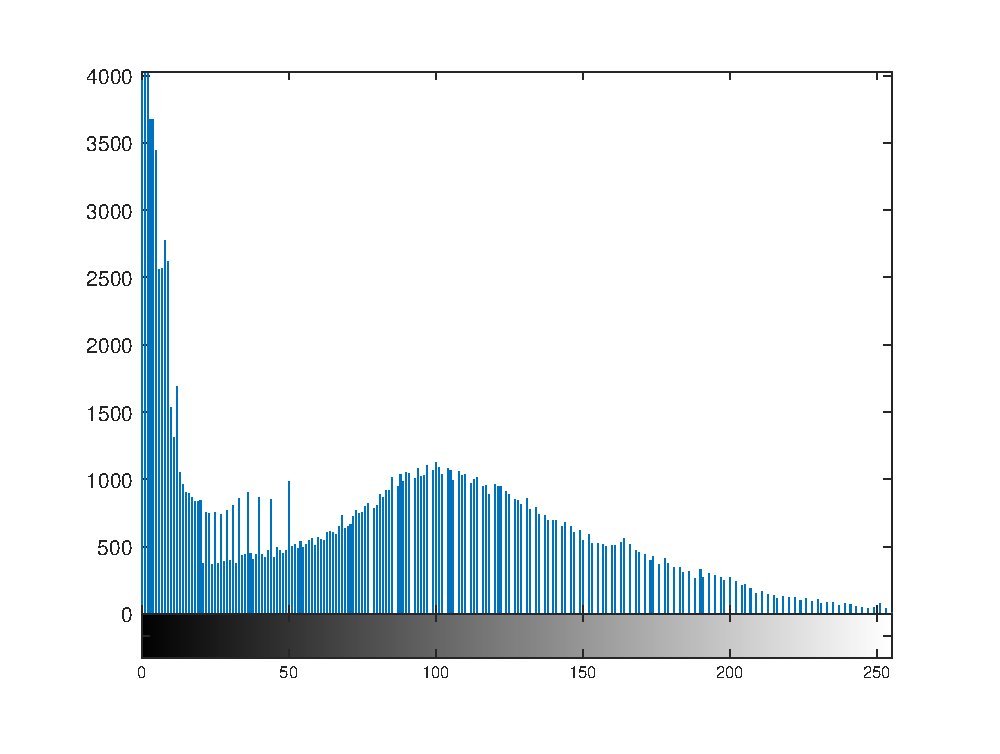
\includegraphics[width=\maxwidth{56.196688409433015em}]{figure_21.eps}
\end{center}
\begin{matlabcode}

figure(6);
imshow(out);
\end{matlabcode}
\begin{center}
\includegraphics[width=\maxwidth{62.117410938283996em}]{figure_22.png}
\end{center}


\matlabheading{Q7 - Histogram Equalization napoleon - Histogram}

\begin{matlabcode}
figure(1);
imhist(I);
\end{matlabcode}
\begin{center}
\includegraphics[width=\maxwidth{56.196688409433015em}]{figure_23.eps}
\end{center}
\begin{matlabcode}

figure(2);
imhist(histeq(I));
\end{matlabcode}
\begin{center}
\includegraphics[width=\maxwidth{56.196688409433015em}]{figure_24.eps}
\end{center}
\begin{matlabcode}

figure(3);
imhist(histeq(Il));
\end{matlabcode}
\begin{center}
\includegraphics[width=\maxwidth{56.196688409433015em}]{figure_25.eps}
\end{center}
\begin{matlabcode}

figure(4);
imhist(histeq(Id));
\end{matlabcode}
\begin{center}
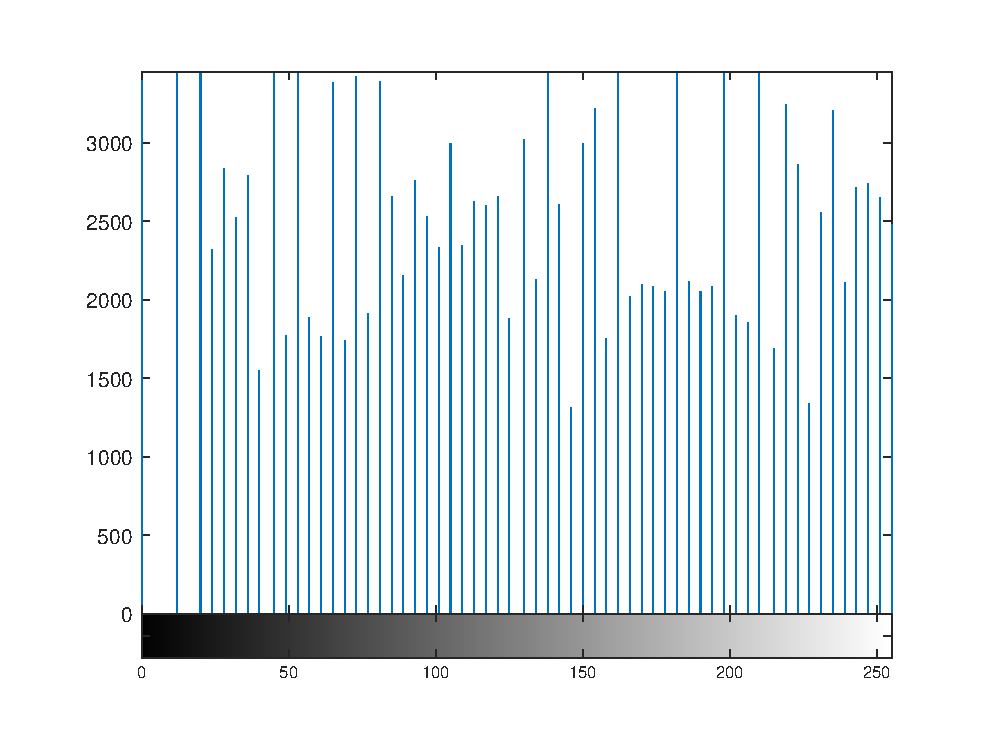
\includegraphics[width=\maxwidth{62.117410938283996em}]{figure_26.eps}
\end{center}


\matlabheading{Q7 - Histogram Equalization napoleon - Images}

\begin{matlabcode}
figure(1);
imshow(I);

figure(2);
imshow(histeq(I));

figure(3);
\end{matlabcode}
\begin{center}
\includegraphics[width=\maxwidth{56.196688409433015em}]{figure_27.png}
\end{center}
\begin{center}
\includegraphics[width=\maxwidth{56.196688409433015em}]{figure_28.png}
\end{center}
\begin{matlabcode}
imshow(histeq(Il));
\end{matlabcode}
\begin{center}
\includegraphics[width=\maxwidth{56.196688409433015em}]{figure_29.png}
\end{center}
\begin{matlabcode}

figure(4);
imshow(histeq(Id));
\end{matlabcode}
\begin{center}
\includegraphics[width=\maxwidth{62.117410938283996em}]{figure_30.png}
\end{center}


\matlabheading{Q7 - Histogram, transform and cumulative histogram - Regular Image}

\begin{matlabcode}
[J,T] = histeq(I);

figure
plot((0:255)/255,T);
\end{matlabcode}
\begin{center}
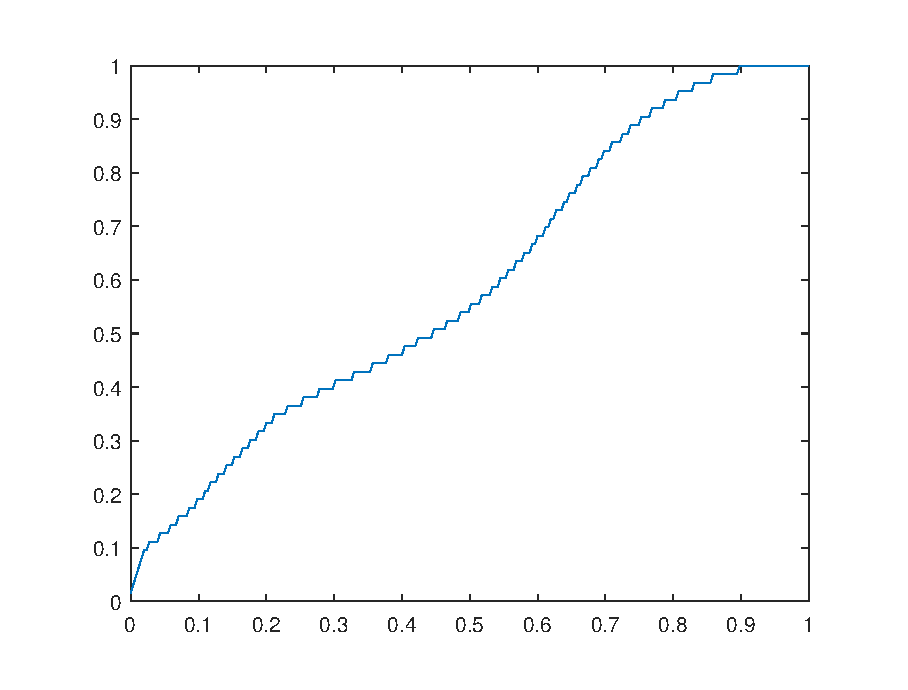
\includegraphics[width=\maxwidth{56.196688409433015em}]{figure_31.eps}
\end{center}
\begin{matlabcode}

figure
plot(cumsum(imhist(I)) / sum(imhist(I)));
\end{matlabcode}
\begin{center}
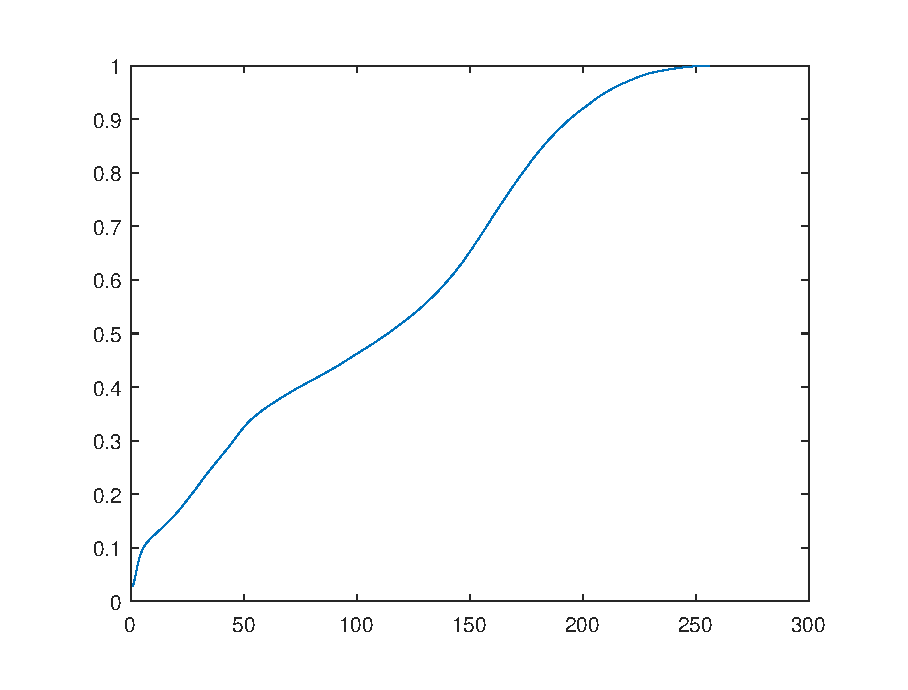
\includegraphics[width=\maxwidth{56.196688409433015em}]{figure_32.eps}
\end{center}
\begin{matlabcode}

figure
plot(cumsum(imhist(J)) / sum(imhist(J)));
\end{matlabcode}
\begin{center}
\includegraphics[width=\maxwidth{56.196688409433015em}]{figure_33.eps}
\end{center}


\matlabheading{Q7 - Histogram, transform and cumulative histogram - Light}

\begin{matlabcode}
[J,T] = histeq(Il);

figure
plot((0:255)/255,T);
\end{matlabcode}
\begin{center}
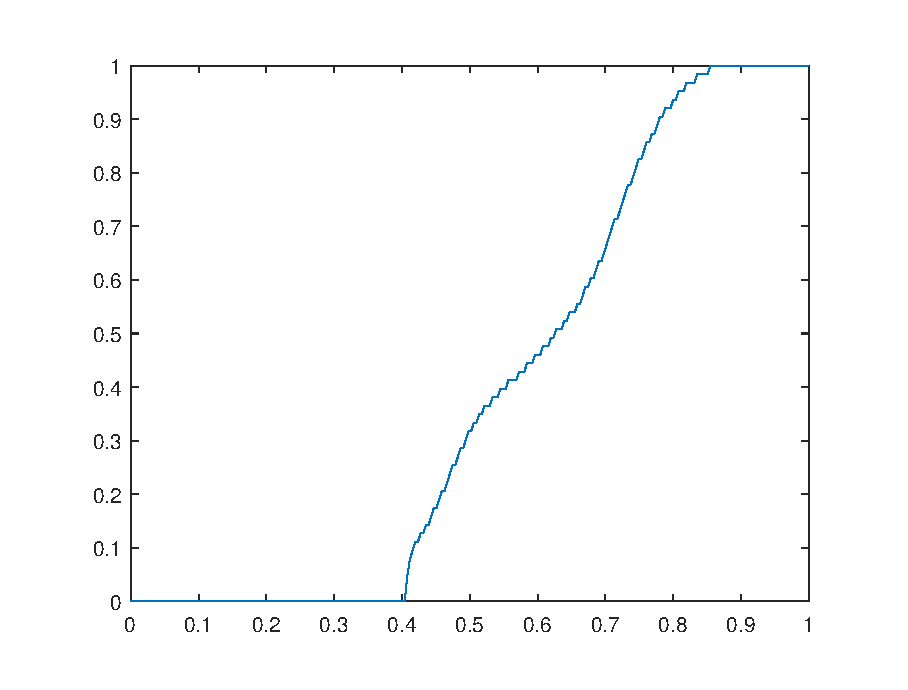
\includegraphics[width=\maxwidth{56.196688409433015em}]{figure_34.eps}
\end{center}
\begin{matlabcode}

figure
plot(cumsum(imhist(Il)) / sum(imhist(Il)));
\end{matlabcode}
\begin{center}
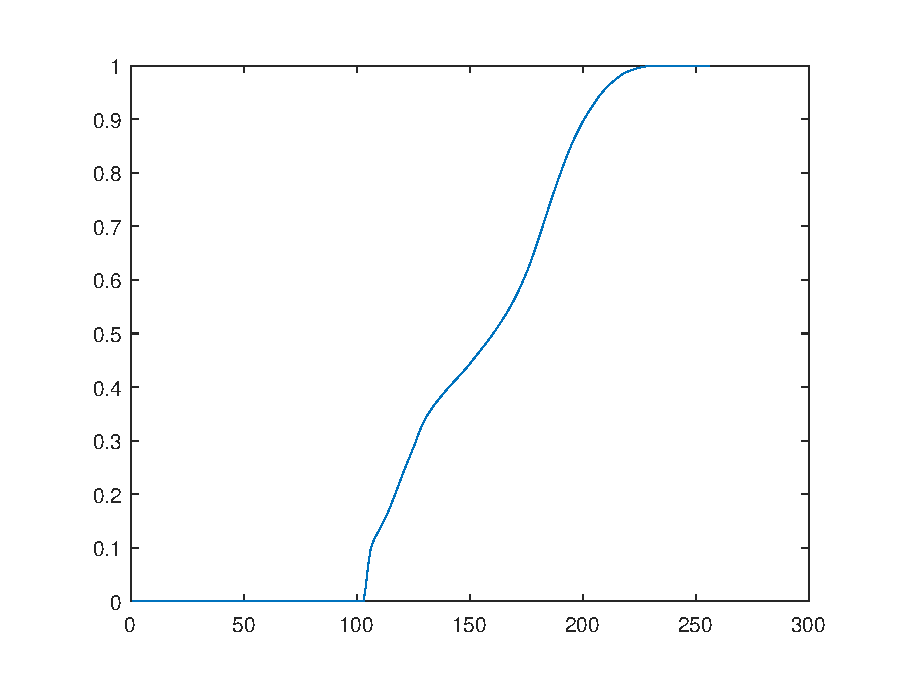
\includegraphics[width=\maxwidth{56.196688409433015em}]{figure_35.eps}
\end{center}
\begin{matlabcode}

figure
plot(cumsum(imhist(J)) / sum(imhist(J)));
\end{matlabcode}
\begin{center}
\includegraphics[width=\maxwidth{56.196688409433015em}]{figure_36.eps}
\end{center}


\matlabheading{Q7 - Histogram, transform and cumulative histogram - Dark}

\begin{matlabcode}
[J,T] = histeq(Id);

figure
plot((0:255)/255,T);
\end{matlabcode}
\begin{center}
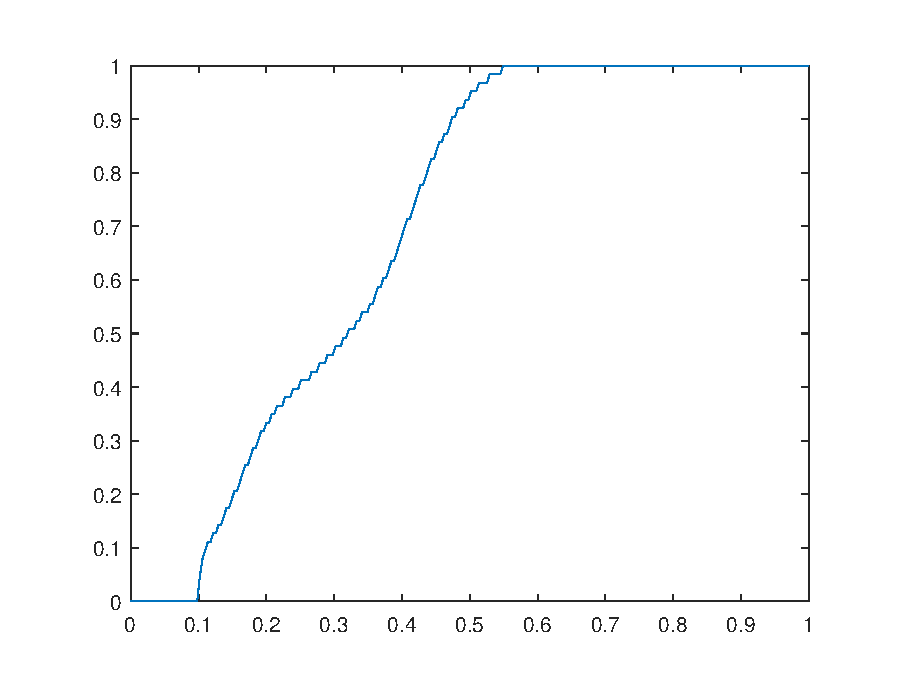
\includegraphics[width=\maxwidth{56.196688409433015em}]{figure_37.eps}
\end{center}
\begin{matlabcode}

figure
plot(cumsum(imhist(Id)) / sum(imhist(Id)));
\end{matlabcode}
\begin{center}
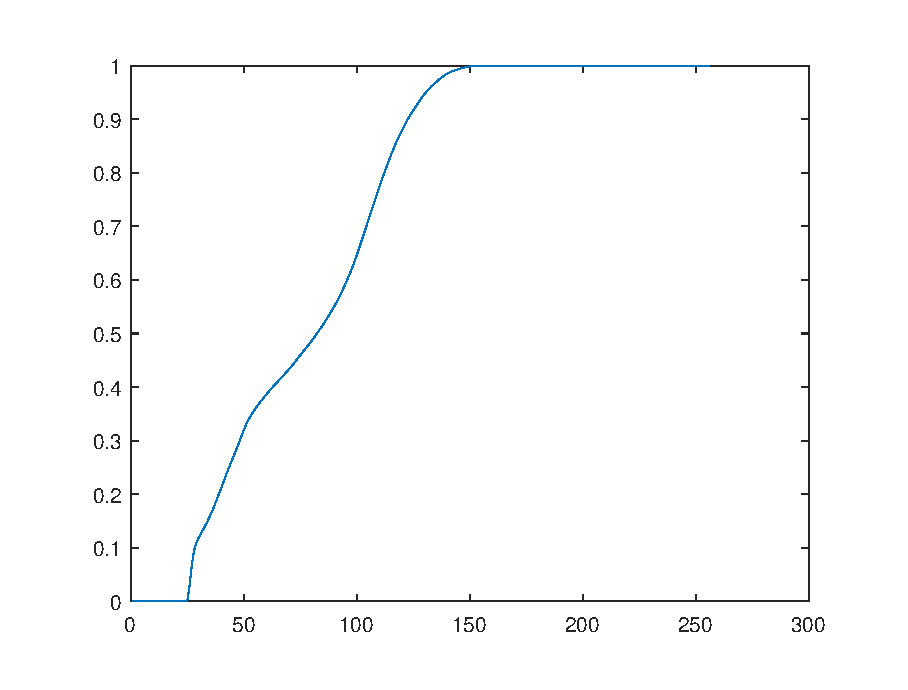
\includegraphics[width=\maxwidth{56.196688409433015em}]{figure_38.eps}
\end{center}
\begin{matlabcode}

figure
plot(cumsum(imhist(J)) / sum(imhist(J)));
\end{matlabcode}
\begin{center}
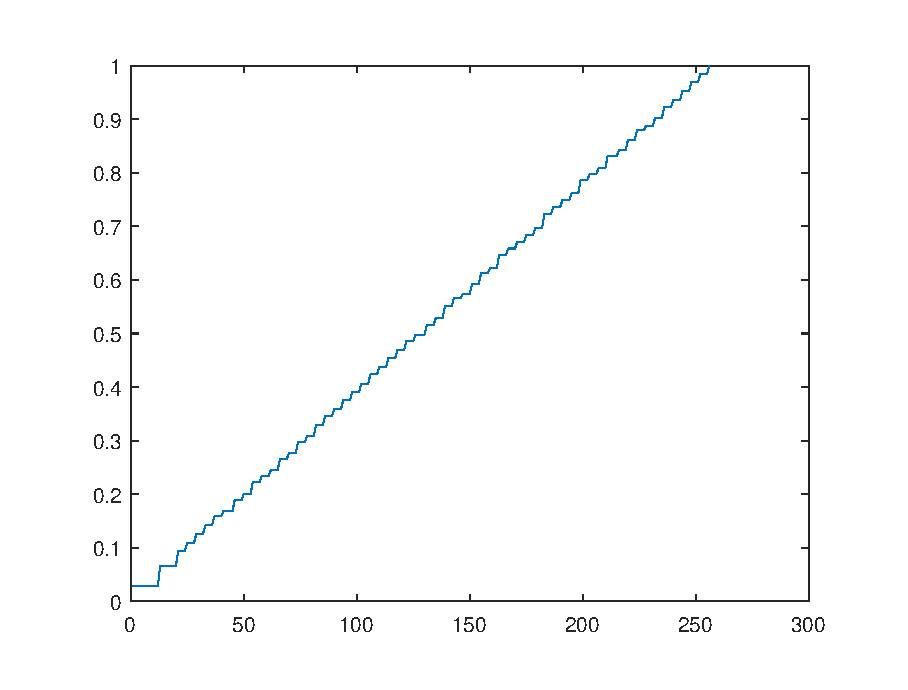
\includegraphics[width=\maxwidth{56.196688409433015em}]{figure_39.eps}
\end{center}


\matlabheading{Q8 - Aliasing when sampling}

\begin{matlabcode}
Jnf = imresize(I, [78 78], 'nearest', 'antialiasing', false);
imshow(Jnf);
\end{matlabcode}
\begin{center}
\includegraphics[width=\maxwidth{25.28850978424486em}]{figure_40.png}
\end{center}
\begin{center}
\includegraphics[width=\maxwidth{56.196688409433015em}]{figure_41.png}
\end{center}
\begin{center}
\includegraphics[width=\maxwidth{56.196688409433015em}]{figure_42.png}
\end{center}

\end{document}
